%% Report layout adapted from the Computer Science report template
%% (Dr Todd R. Jones, University of Reading, based on a template by Dr Varun Ojha),
%% as required by the course. The template's CS_report.sty settings are included
%% below so that the whole report lives in this file.
\documentclass[a4paper,11pt,oneside]{book}

%% ----- Template settings (CS_report.sty) -----
\usepackage[margin=1.2in]{geometry}

% Sans-serif font
\usepackage[T1]{fontenc}
\usepackage{lmodern}
\renewcommand*\familydefault{\sfdefault}
\usepackage{slantsc}
\usepackage{relsize}
\usefont{T1}{lmss}{m}{n}\selectfont
\DeclareFontShape{T1}{lmss}{m}{sc}{<->ssub*lmss/m/n}{}

% Math
\usepackage{sansmath}
\sansmath
\usepackage[cmex10]{amsmath}
\usepackage{amssymb}
\usepackage{amsthm}

% Code listings
\usepackage[utf8]{inputenc}
\usepackage{listings}
\usepackage{xcolor}
\definecolor{codegreen}{rgb}{0,0.6,0.1}
\definecolor{codegray}{rgb}{0.5,0.5,0.5}
\definecolor{codeblue}{rgb}{0.10,0.00,1.00}
\definecolor{codepurple}{rgb}{0.58,0,0.82}
\definecolor{backcolour}{rgb}{1.0,1.0,1.0}
\lstdefinestyle{mystyle}{
    backgroundcolor=\color{backcolour},
    commentstyle=\color{codegreen},
    keywordstyle=\color{codeblue},
    numberstyle=\tiny\color{codegray},
    stringstyle=\color{codepurple},
    basicstyle=\ttfamily\footnotesize,
    breakatwhitespace=false,
    breaklines=true,
    captionpos=b,
    keepspaces=true,
    numbers=left,
    numbersep=5pt,
    showspaces=false,
    showstringspaces=false,
    showtabs=false,
    tabsize=2,
    frame=none
}
\lstset{style=mystyle}

% Figures and tables
\usepackage{graphicx}
\usepackage{caption}
\usepackage{multirow}
\usepackage{rotating}
\usepackage{makecell}
\usepackage{booktabs}

% List of abbreviations
\usepackage{enumitem}
\newlist{abbrv}{itemize}{1}
\setlist[abbrv,1]{label=,labelwidth=1in,align=parleft,itemsep=0.1\baselineskip,leftmargin=!}

% Links and references
\usepackage[hidelinks]{hyperref}
\usepackage[nameinlink]{cleveref}
\definecolor{DarkBlue}{rgb}{0.00,0.00,0.50}
\hypersetup{colorlinks=true,
            linkcolor=blue,
            filecolor=magenta,
            urlcolor=cyan,
            citecolor=DarkBlue,
            pdftitle={Tsunami Monitoring System -- Workshop 3},
            }

% Bibliography: the template's numbered style (natbib numbers)
\usepackage[numbers]{natbib}
\usepackage[nottoc]{tocbibind}
\renewcommand{\bibname}{References}

% Appendices
\usepackage[toc]{appendix}

%% ----- Additions for this report -----
\usepackage{tabularx}
\usepackage{float}
\usepackage{tikz}
\usetikzlibrary{arrows.meta,calc,positioning}
\newcolumntype{Y}{>{\raggedright\arraybackslash}X}
\newcolumntype{L}[1]{>{\raggedright\arraybackslash}p{#1}}
\newcommand{\goldstamp}{\texttt{20261120\_060020}}
\newcommand{\golddate}{20 November 2026, 06:00:20 UTC}
\newcommand{\manualgoldstamp}{\texttt{20261120\_044653}}
\newcommand{\dbdate}{20 November 2026, 05:23:51 UTC}
\hypersetup{bookmarksdepth=1}
\renewcommand{\arraystretch}{1.25}
% Long file names and code words: allow looser lines and breaks in paths at _ and .
\setlength{\emergencystretch}{3em}
\expandafter\def\expandafter\UrlBreaks\expandafter{\UrlBreaks\do\_\do\.}

\begin{document}

    \captionsetup[figure]{margin=1.5cm,font=small,name={Figure},labelsep=colon}
    \captionsetup[table]{margin=1.5cm,font=small,name={Table},labelsep=colon}

    \frontmatter

    % -------------------------------------------------------------------
    % Title page
    % -------------------------------------------------------------------
    \begin{titlepage}
        \begin{center}
            
\includegraphics[width=3cm]{figures/ud.png}\\[0.5cm]
            {\LARGE Universidad Distrital Francisco Jos\'e de Caldas\\[0.5cm]
            School of Engineering -- Computer Engineering Program}\\[2cm]

            \linespread{1.2}\huge {
                Tsunami Monitoring System\\[0.3cm]
                \Large Workshop No.\ 3: Pipeline Improvements, Incremental Ingestion and Gold Layer
            }
            \linespread{1}~\\[2cm]

            {\Large Team 8}\\[0.5cm]
            {\large
            \begin{tabular}{ll}
                Lina Moreno & 20231020133 \\
                Jaider \'Avila & 20231020200 \\
                Gabriela Mart\'inez & 20231020205 \\
            \end{tabular}}\\[1cm]

            {\large \emph{Professor:} Eng.\ Carlos Andr\'es Sierra, M.Sc.}\\[1cm]

            \large A report submitted for Workshop No.\ 3 of the course\\
            \textit{Data Analysis Programming}, Semester 2026-II\\[0.3cm]
            \small
            Repository: \url{https://github.com/g8martinezsilva/tsunami-monitoring}\\[0.2cm]
            Branch: \texttt{feat/workshop3-incremental-gold}
            \vfill

            \today
        \end{center}
    \end{titlepage}

    % -------------------------------------------------------------------
    % Declaration
    % -------------------------------------------------------------------
    \newpage
    \thispagestyle{empty}
    \chapter*{\Large Declaration}
    We, Lina Moreno, Jaider \'Avila and Gabriela Mart\'inez, of the Computer Engineering Program, Universidad Distrital Francisco Jos\'e de Caldas, confirm that this is our own work and that figures, tables, equations, code snippets and illustrations in this report are original and have not been taken from any other person's work, except where the works of others have been explicitly acknowledged, quoted, and referenced. Data from external sources are cited with their licenses.
    ~\\[1cm]
    \begin{flushright}
    Lina Moreno\\
    Jaider \'Avila\\
    Gabriela Mart\'inez

    \today
    \end{flushright}

    % -------------------------------------------------------------------
    % Abstract (executive summary)
    % -------------------------------------------------------------------
    \chapter*{Abstract}
    \addcontentsline{toc}{chapter}{Abstract}
The Team~8 Tsunami Monitoring System combines earthquake catalogs, historical tsunami records, and official warning-center messages for a Pacific monitoring analyst. Workshop~3 extends the Workshop~2 Bronze and Silver workflow with scheduled feed polling, source-aware revision detection and committed watermarks. The loader preserves one observation per source and external identifier while retaining raw evidence and quarantine records. PostGIS evaluates cross-source links and keeps ambiguous cases for review.

A local PySpark task selects current versions across Silver snapshots and writes two Parquet datasets. Governance describes processing volume, completeness and validation outcomes. Storytelling provides yearly counts, measurement distributions and bulletin coverage. The selected Gold pair consolidates 2,912 observations across five sources. Thirteen recorded incremental source loads contained three inserted observations and four business updates.

In the NOAA subset, 32 observations have a known date and an incomplete timestamp. The 209 available maximum water heights have a median of 0.20~m and a mean of 6.42~m, reflecting the long upper tail. Among 172 records classified as earthquake-caused with both measurements, reported earthquake magnitude and maximum water height show a positive rank association (Spearman $\rho=0.471$).

    % -------------------------------------------------------------------
    % Contents, list of figures, list of tables, abbreviations
    % -------------------------------------------------------------------
    \setcounter{tocdepth}{0}
    \tableofcontents
    \setcounter{tocdepth}{1}
    \listoffigures
    \listoftables

    \chapter*{List of Abbreviations}
    \chaptermark{List of Abbreviations}
    \begin{abbrv}
        \item[CAP]      Common Alerting Protocol
        \item[DAG]      Directed Acyclic Graph (Airflow workflow)
        \item[EDA]      Exploratory Data Analysis
        \item[FDSN]     International Federation of Digital Seismograph Networks
        \item[HazEL]    NCEI Hazard Event Database (Global Historical Tsunami Database interface)
        \item[IQR]      Interquartile Range
        \item[NCEI]     NOAA National Centers for Environmental Information
        \item[NOAA]     National Oceanic and Atmospheric Administration
        \item[NTWC]     National Tsunami Warning Center (Palmer, Alaska)
        \item[KPI]      Key Performance Indicator
        \item[PTWC]     Pacific Tsunami Warning Center (Honolulu, Hawaii)
        \item[USGS]     United States Geological Survey
        \item[UTC]      Coordinated Universal Time
    \end{abbrv}

    % -------------------------------------------------------------------
    % Main chapters
    % -------------------------------------------------------------------
    \mainmatter


\chapter{Introduction}
\label{ch:intro}
The system helps a Pacific coastal monitoring analyst examine earthquake observations, historical tsunamis, and official warning-center messages together. NOAA HazEL provides the historical tsunami catalog, USGS supplies a historical earthquake catalog and a recent-event feed, and NTWC and PTWC publish Atom entries that link to Common Alerting Protocol (CAP) messages. The earlier workshops define the source contracts, traceability rules and analyst decisions that guide these choices \cite{workshop1,workshop2,hazel,usgsfdsn,usgsfeed,tsunamigov}.

The 2026-II course specification places scheduled incremental ingestion, watermarks, idempotency, and cross-source event identification in Workshop~3. Team~8 applies those requirements to earthquake and tsunami correlation. The 2026-I Gold guide informs the use of PySpark and the two analytical datasets. This implementation uses the structured seismic, geographic, and alert fields available for this assignment. The monitoring dashboard belongs to Workshop~4 \cite{courseproject,teamassignment,goldguide}.

Figure~\ref{fig:w3-architecture} extends the Workshop~2 flow. PostgreSQL stores canonical observations and links. Gold reads saved Silver Parquet to compute indicators independently of the database load. The CLI can invoke the shared ingestion functions directly.

\begin{figure}[H]
\centering
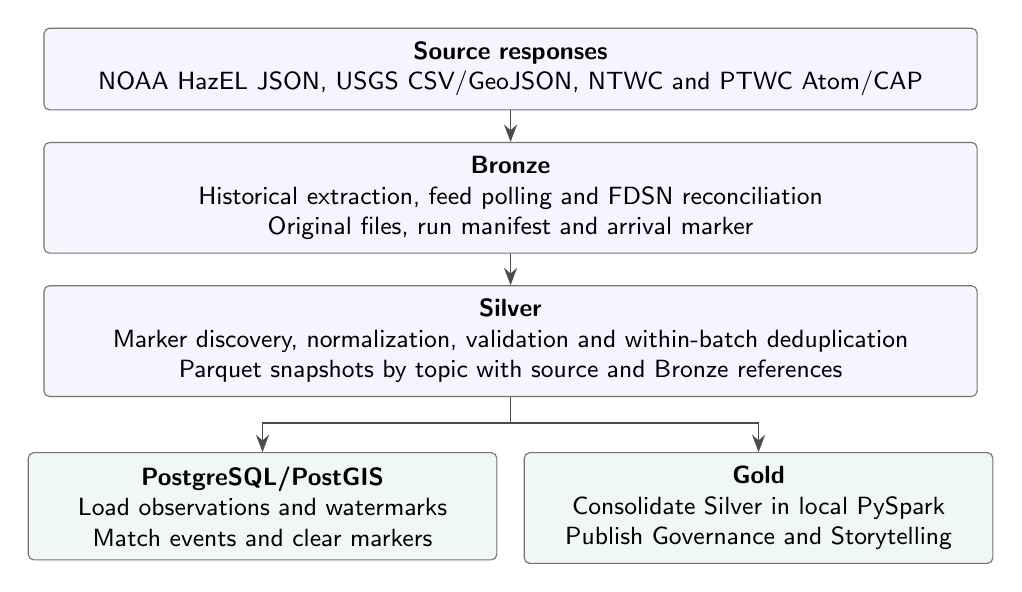
\begin{tikzpicture}[
    node distance=4mm,
    flowbox/.style={draw=black!55, rounded corners=2pt, align=center,
        font=\small, inner sep=5pt, fill=blue!4, text width=11.5cm},
    outputbox/.style={flowbox, fill=teal!6, text width=5.6cm, anchor=north},
    flow/.style={-{Stealth[length=2.2mm]}, semithick, draw=black!70}
]
\node[flowbox] (src) {\textbf{Source responses}\\
    NOAA HazEL JSON, USGS CSV/GeoJSON, NTWC and PTWC Atom/CAP};
\node[flowbox, below=of src] (bronze) {\textbf{Bronze}\\
    Historical extraction, feed polling and FDSN reconciliation\\
    Original files, run manifest and arrival marker};
\node[flowbox, below=of bronze] (silver) {\textbf{Silver}\\
    Marker discovery, normalization, validation and within-batch deduplication\\
    Parquet snapshots by topic with source and Bronze references};
\node[outputbox] (db) at ($(silver.south)+(-3.15,-0.70)$) {\textbf{PostgreSQL/PostGIS}\\
    Load observations and watermarks\\
    Match events and clear markers};
\node[outputbox] (gold) at ($(silver.south)+(3.15,-0.70)$) {\textbf{Gold}\\
    Consolidate Silver in local PySpark\\
    Publish Governance and Storytelling};
\draw[flow] (src) -- (bronze);
\draw[flow] (bronze) -- (silver);
\draw[flow] (silver.south) -- ++(0,-0.33) -| (db.north);
\draw[flow] (silver.south) -- ++(0,-0.33) -| (gold.north);
\end{tikzpicture}
\caption[Workshop 3 pipeline]{Workshop~3 pipeline on Docker Compose. Airflow orchestrates scheduled and manual runs. The CLI invokes the shared ingestion path with its own manifests.}
\label{fig:w3-architecture}
\end{figure}

\chapter{Pipeline Improvements}
\label{ch:pipeline}

\section{Observations from Workshop 2}
Workshop~2 already implemented the manual Bronze DAG, the Silver FileSensor, WGS84 coordinate normalization, source-specific validation and quarantine, IQR flags, and PostgreSQL upserts keyed by source and external ID. The historical loader already committed source state with the data. Its Silver samples made repeated historical processing visible. Workshop~1 also documented changes in USGS observations over time, incomplete NOAA time fields, and inconsistencies in CAP timestamps. These observations motivated source-aware revision checks and explicit review criteria for relationships \cite{workshop1,workshop2}.

\section{Incremental Ingestion and Watermarks}
The \path{incremental_ingestion} DAG polls the USGS real-time, NTWC and PTWC feeds every ten minutes. USGS offers a rolling 30-day GeoJSON feed. The warning-center tasks parse each available Atom entry and fetch its linked CAP message. The polling code normalizes the rows in memory with the Silver helpers and compares each external ID against its committed PostgreSQL version. This allows an unseen ID to enter even when its update timestamp precedes the source watermark. Comparing the CAP payload also detects a correction with the same issue time \cite{airflow,usgsfeed,tsunamigov}.

The \path{usgs_fdsn_reconciliation} DAG is configured for a daily catalog query. It reads the committed FDSN revision watermark and queries the catalog with \path{updatedafter} set to 24 hours before that value. The query specifies an origin-time start of 1 January 2010 so that older earthquakes can be included when revised. The count endpoint is used to check the returned CSV. The historical load supplies the first FDSN watermark, and the reconciliation skips the query when that state is absent \cite{usgsfdsn}.

A feed response enters Bronze when it contains a new observation, a business or revision-metadata change, or a rejected record. The original response remains available in full. A valid set of files produces a Bronze manifest and an arrival marker for the Silver sensor. Silver preprocesses the files named in that manifest, writes its Parquet and passes the outputs to the loader. Logs and manifests provide evidence for extraction, while \path{ingestion_run} provides evidence for successful source loads. The recorded examples in \cref{tab:incremental-runs,tab:airflow-examples} demonstrate the difference.

\section{Change Detection and Duplicate Handling}
The loader compares normalized business fields through a SHA-256 hash and tracks revision metadata separately. For USGS, \path{source_updated_at} protects the committed observation from an older revision. For CAP, the comparison uses Atom update times when both versions supply them and issue times otherwise. A change to revision metadata alone can advance the stored metadata while leaving the business update count unchanged. NOAA HazEL supplies a historical catalog without a source revision watermark in this pipeline.

Each source load writes the canonical \path{event} row and its domain attributes within one transaction. The \path{UNIQUE(source, external_id)} constraint and \path{ON CONFLICT} preserve the observation's identity on an update. The source's counters and watermark commit with the data, and the watermark is monotonic. USGS uses the revision time and CAP uses the issue time. The counter \path{unchanged_count} also covers stale and metadata-only rows that produced no business update. The Workshop~3 migration adds this counter to existing Workshop~2 volumes \cite{postgresql}.

Quarantine still records the source, reason and Bronze locator. Reloading the same Bronze reference and reason preserves one quarantine entry, while the processing counters record each rejection occurrence. After a successful PostgreSQL load, Silver runs matching before clearing its marker. A failed matching task can therefore be retried with the committed load and saved artifacts.

\section{Event Identification Across Sources}
The matcher evaluates time, geography, source attributes and identity evidence in \path{src/matching.py}. PostGIS computes distances on geographic coordinates. The project uses the 15-minute and 100~km exploratory limits from Workshop~1 as the NOAA candidate window for complete timestamps. Narrower acceptance limits add a safeguard against plausible but ambiguous matches. The configured windows are heuristics for this dataset \cite{workshop1,postgis-distance}.

\begin{table}[!htbp]
\centering
\small
\begin{tabularx}{\textwidth}{@{}L{2.9cm}YY@{}}
\toprule
Observation & Candidate conditions & Automatic acceptance \\
\midrule
NOAA with seconds & Within 15 minutes and 100~km. The catalog cause must be earthquake-related. Known validity must be positive. When both earthquake magnitudes are available, the difference is at most 0.5. & A single distinct USGS ID, within 120~s and 25~km, with both magnitudes agreeing. The NOAA cause must be earthquake only and validity probable or definite. \\
NOAA with a partial time & Within the recorded minute, hour or calendar day and 100~km. The same cause and validity conditions apply. Hour and day records require both earthquake magnitudes to agree within 0.5. & Pending review. \\
NTWC or PTWC CAP & Within 120~s of the CAP-reported earthquake origin and 100~km. Check the 0.5 magnitude tolerance when both are available. & A single distinct USGS ID, within 25~km, and both magnitudes agree within 0.5 and use the same reported type. \\
USGS FDSN and Realtime & The same USGS external ID for earthquake observations. & Group the two observations when membership and review evidence are compatible. \\
\bottomrule
\end{tabularx}
\caption[Candidate and acceptance rules]{Candidate and acceptance rules in \texttt{config/sources.yaml} and \texttt{src/matching.py}, rule version~2.}
\label{tab:matching-policy}
\end{table}

For partial NOAA times, the matcher constructs a search interval with an exclusive upper bound. The stored timestamp remains null. The magnitude comparison uses the earthquake magnitude reported by NOAA or CAP alongside USGS earthquake magnitude. Maximum water height is a separate measurement. If several distinct USGS IDs qualify, the candidates stay pending.

Verified identity is expressed through \path{event_group} membership while retaining both source records. A \path{caused_by} link connects a tsunami observation to a candidate earthquake and a \path{reports_on} link connects a bulletin to the earthquake it describes. Accepted links indicate that the evidence meets the project rule. Scientific attribution requires independent evidence. Reconciliation reassesses automatic links when their inputs change. Contradictory data can invalidate a link, missing inputs can return it to review, and explicit manual decisions are preserved.

\section{Silver Layer Changes}
Silver writes four topic directories for earthquakes, tsunami events, bulletins and rejected records, with a separate manifest that records file paths and row counts. Each row keeps its Bronze filename and locator. New Parquet timestamps use microsecond resolution for Spark compatibility. NOAA calendar dates and recorded clock components remain available for partial times. Archived Workshop~2 files in the Silver root are included in Gold through the compatibility step in \cref{sec:gold-transforms} \cite{parquet}.

\section{Before and After Summary}
\begin{table}[!htbp]
\centering
\footnotesize
\begin{tabularx}{\textwidth}{@{}L{1.8cm}YYYY@{}}
\toprule
Component & Workshop 2 & Workshop 3 & Reason & Evidence \\
\midrule
Extraction & Manual historical DAG with feed snapshots. & Scheduled feed scans plus a daily FDSN DAG. & Find new observations and later revisions. & DAG definitions and \cref{tab:airflow-examples}. \\
Versioning & UPSERT and business hash on the canonical key. & Per-ID polling, stale-revision checks and separate metadata handling. & Preserve the current version and distinguish a business change. & \path{src/load.py} and \cref{tab:incremental-runs}. \\
State and quarantine & Per-source transactions, historical load watermarks and rejection references. & Scheduled use of committed watermarks, timestamp comparisons and explicit unchanged counts. & Make replay and source processing outcomes visible. & \path{sql/03_workshop3.sql}, \path{ingestion_state}. \\
Silver files & Flat Parquet files per run. & Topic directories and Spark-compatible timestamps. & Collect several snapshots per topic with compatible types. & Saved Silver manifests and \cref{sec:gold-transforms}. \\
Matching & Exploratory associations and a canonical grouping model. & Reviewable links, exact-ID grouping and reassessment of revisions. & Preserve evidence when relationships change. & Rule configuration and \cref{tab:relations}. \\
Analytics & Silver exploration in pandas. & PySpark consolidation and two published Gold datasets. & Separate the current observation counts from processing history. & \cref{tab:gold-quality,tab:story-counts} and the notebook. \\
\bottomrule
\end{tabularx}
\caption{Changes from Workshop~2 and the artifacts used to verify them.}
\label{tab:before-after}
\end{table}

\chapter{Data Quality Findings}
\label{ch:quality}
The pandas notebook \path{notebooks/03_data_quality.ipynb} uses the published Gold pair \goldstamp{} for source coverage and Governance. For individual NOAA measurements, it reads the Workshop~3 topic snapshots and the flat Workshop~2 Silver archives. It selects the latest Bronze capture per source key, with Silver processing time and the file stamp as fallbacks, following the version ordering in \cref{sec:gold-transforms} \cite{pandas}.

The EDA starts with completeness, uniqueness and validity checks, then examines the height distribution, yearly coverage and the magnitude--height association \cite[PDF pp.~14, 23, 26 and 31]{edaguide}.

\begin{table}[htbp]
\centering
\small
\begin{tabular}{@{}lrrrrrr@{}}
\toprule
Source & \makecell{Silver rows\\processed} & \makecell{Unique\\observations} & \makecell{Repeated\\rows} &
    \makecell{Missing\\coordinates} & \makecell{Incomplete\\time} & \makecell{IQR\\flags} \\
\midrule
USGS FDSN     & 3,863 & 1,929 & 1,934 & 0 & 0  & 323 \\
USGS Realtime & 11,304 &  759 & 10,545 & 0 & 0 & 117 \\
NOAA HazEL    &   459 &   221 &   238 & 9 & 32 &  33 \\
NTWC          &     3 &     1 &     2 & 0 & 0  & -- \\
PTWC          &     3 &     2 &     1 & 0 & 0  & -- \\
\bottomrule
\end{tabular}
\caption[Observation counts and quality flags from Governance]{Observation counts and quality flags from Governance, published \golddate. Completeness counts and inherited Silver IQR flags use the selected observations. The dash marks a topic without an IQR measure.}
\label{tab:gold-quality}
\end{table}

Governance counts 15,632 processed observation rows and 2,912 distinct source keys across five sources. The 12,720 additional rows include repeated captures and revisions. A single physical earthquake can appear in both USGS catalogs.

Of 221 NOAA observations, nine lack at least one coordinate (4.07\%), 12 lack a finite maximum water height (5.43\%), and 32 lack a full timestamp (14.48\%). The partial timestamps comprise 23 date-only and nine minute-precision records. They contribute to yearly counts and widen the time interval considered in matching. Recorded NOAA clock components are treated as UTC under the Workshop~1 assumption \cite{workshop1}.

All recorded NOAA coordinates are within the normalized bounds. Across the saved Silver CAP snapshots, one of three bulletin identifiers has a snapshot with expiry before issue. Governance counts two FDSN rejection occurrences and one distinct rejection. The earlier PostgreSQL check found one quarantine record with reason \texttt{event type nuclear explosion} and zero duplicate canonical source keys (\cref{ch:results}).

\section{Tsunami Water Heights}
\Cref{tab:noaa-height-stats} summarizes finite maximum water heights from the 221 consolidated NOAA observations. The median of 0.20~m and the middle half from 0.08 to 0.70~m describe the centre and spread. The mean of 6.42~m is sensitive to the large measurements in the upper tail (\cref{fig:noaa-heights}).

\begin{table}[htbp]
\centering
\small
\begin{tabular}{@{}lr@{\hspace{2em}}lr@{}}
\toprule
Statistic & Value & Statistic & Value \\
\midrule
Finite heights & 209 & Minimum & 0.00~m \\
Mean & 6.42~m & Maximum & 481.00~m \\
Median & 0.20~m & Sample standard deviation & 38.36~m \\
First quartile & 0.08~m & Third quartile & 0.70~m \\
Interquartile range & 0.62~m & & \\
\bottomrule
\end{tabular}
\caption{Descriptive statistics of maximum water height in the selected NOAA HazEL records.}
\label{tab:noaa-height-stats}
\end{table}

\begin{figure}[htbp]
\centering
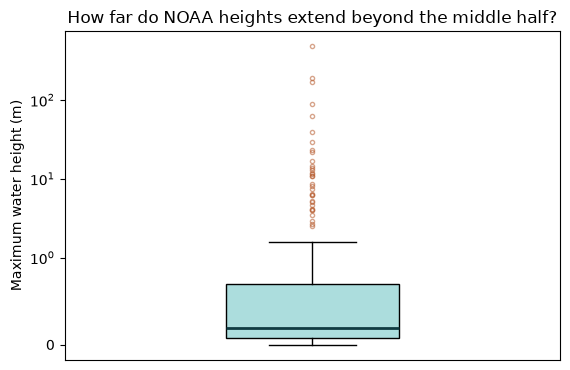
\includegraphics[width=.78\textwidth]{figures/noaa_water_height_boxplot.png}
\caption[Distribution of NOAA maximum water heights]{Distribution of maximum water height in 209 NOAA observations. The axis is linear up to 1~m and logarithmic above it so the box and extreme values remain visible.}
\label{fig:noaa-heights}
\end{figure}

The notebook recomputes the IQR fences on the consolidated measurements, using $Q_1-1.5\,\mathrm{IQR}$ and $Q_3+1.5\,\mathrm{IQR}$. Governance reports the flags inherited from the original Silver batches. In the consolidated set, 33 heights exceed the upper fence. The largest is 481~m at Tracy Arm, Alaska (NOAA record 6045). The summary retains all finite measurements and uses the flags to identify cases for review \cite[PDF pp.~16--19 and 27--30]{edaguide}.

\chapter{Governance KPIs}
\label{ch:governance}
Gold writes one observation summary per topic and source, plus a rejection summary per source where rejection rows exist. In \cref{tab:kpis}, $N$ is the number of unique observations for an observation summary. The two rates divide by $N$ and are rounded to two decimal places. \Cref{tab:gold-quality} gives the measured counts that motivate the indicators.

\begin{table}[!htbp]
\centering
\small
\begin{tabularx}{\textwidth}{@{}L{4.2cm}Y@{}}
\toprule
Indicator & Computation and interpretation \\
\midrule
\path{rows_processed} & Count all observation rows read for the topic and source. Both repeated copies and revisions contribute to processing volume. \\
\path{unique_observations} & Count selected source and external ID keys. This measures source coverage. Two catalogs may report the same event. \\
\path{repeated_rows} & Subtract $N$ from \path{rows_processed} to count additional occurrences in saved batches, including valid revisions. \\
\path{missing_coordinates} & Count current rows missing either coordinate, including NaN values. This identifies incomplete geographic input. \\
\path{missing_coordinates_pct} & $100 \times$ missing-coordinate count divided by $N$. This measures geographic completeness by topic and source. \\
\path{incomplete_times} & Count current rows without \path{event_time}, or without \path{sent_at} for CAP. A NOAA row may still contain a date. \\
\path{incomplete_times_pct} & $100 \times$ incomplete-time count divided by $N$. This measures timestamp completeness by topic and source. \\
\path{rejected_records} & Count all saved rejection rows by source. Replaying a raw record can add another rejection occurrence. \\
\path{unique_rejected_records} & Count distinct source, external ID, Bronze filename, locator and reason combinations. The raw reference supports counting rejections with missing IDs. \\
\path{iqr_outliers} & Count current rows with a Silver depth (km) or water-height (m) flag. The result depends on the original batch distribution. \\
\bottomrule
\end{tabularx}
\caption{Implemented Governance indicators. Rejection counts use the saved rejection history and observation completeness uses the selected version of each key.}
\label{tab:kpis}
\end{table}

\chapter{Storytelling Aggregations}
\label{ch:storytelling}
\section{Aggregations}
Storytelling aggregates the selected Silver observations by source and the dimension of each metric. The reported magnitude type is retained and magnitude intervals have width 0.5. Water-height intervals have width 1~m. Both use inclusive lower bounds and exclusive upper bounds, and the distributions use finite values. The totals in \cref{tab:story-counts} describe the coverage of each separate metric.

\begin{table}[htbp]
\centering
\small
\begin{tabularx}{\textwidth}{@{}L{3.1cm}YY@{}}
\toprule
Indicator & Grouping & Contribution to Workshop~1 user stories \\
\midrule
Earthquakes by year & Source and UTC year of the reported origin, when available. & Gives US3 a view of the historical catalog's coverage and context for recent records. \\
Historical tsunamis by year & NOAA source and calendar year, using the preserved event date when available. & Gives US3 a record of reported tsunami observations by year. \\
Earthquake magnitude distribution & Source, magnitude type and half-open magnitude interval. & Helps US3 see which parts of the magnitude range each catalog covers. \\
Maximum tsunami water-height distribution & NOAA source and half-open interval in metres. & Adds historical context to US3 about the reported water-height measurements. \\
Bulletins by center & Source and issuing center. & Shows the available NTWC and PTWC message coverage for US2. The bulletin details and earthquake links are in PostgreSQL. \\
\bottomrule
\end{tabularx}
\caption{Storytelling aggregations and their contributions to the analyst tasks defined in Workshop~1 \cite{workshop1}.}
\label{tab:story-purpose}
\end{table}

\section{Dashboard Narrative}
A coastal analyst can first examine how much each source contributes and how complete its observations are. The historical counts and distributions then provide context for a new observation. Governance contributes to the data-quality story US6. The run records and CLI status provide freshness evidence for US5. Looking up recent events on a map and presenting a tsunami-relevance indicator belong to the later dashboard \cite{workshop1,courseproject}.

\begin{figure}[htbp]
\centering
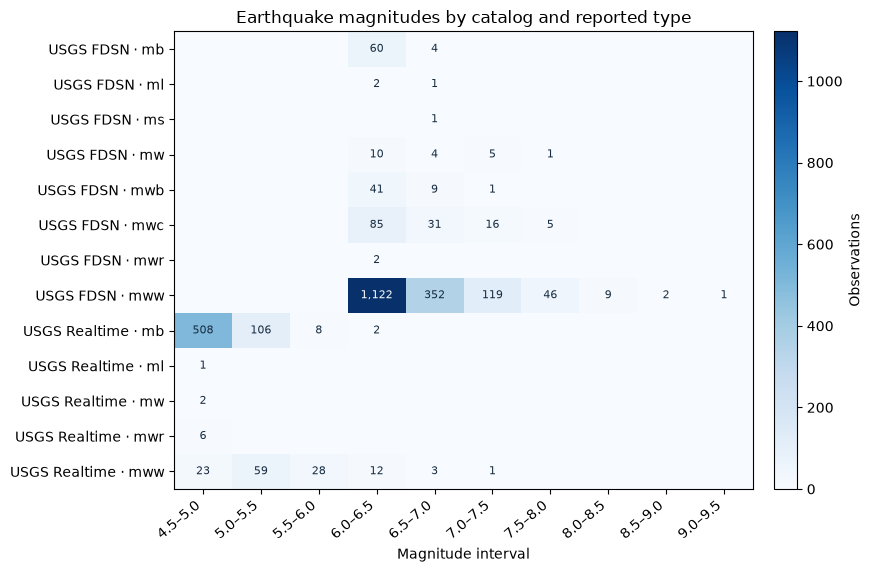
\includegraphics[width=\textwidth]{figures/gold_earthquake_magnitudes.png}
\caption[Earthquake magnitude by catalog and reported type]{Earthquake observations by source, reported magnitude type and numeric interval in Gold pair \goldstamp. Blank cells denote zero observations.}
\label{fig:magnitudes}
\end{figure}

The notebook's heatmap (\cref{fig:magnitudes}) shows a concentration of 1,122 \texttt{mww} observations in $[6.0,6.5)$ for FDSN and 508 \texttt{mb} observations in $[4.5,5.0)$ for Realtime. The FDSN historical query covers a broad Pacific bounding box with $M\geq 6$, and its observations in this pair span 2010--2025. Realtime uses the $M\geq 4.5$ rolling feed and the retained snapshots contribute observations from 2026. A comparison of seismic activity would require a common geographic selection, magnitude criterion and temporal baseline \cite{usgsfdsn,usgsfeed}.

\section{Exploratory Tsunami Findings}
\subsection{Annual NOAA Coverage}
The notebook groups the 221 consolidated NOAA observations by recorded calendar year from 2010 through 2025, including dated records with incomplete clocks. A line chart shows differences between years \cite[PDF pp.~49--52]{edaguide}. The count ranges from eight in 2020 to 18 in both 2022 and 2025. The variation describes the Pacific subset queried from HazEL \cite{hazel,workshop1}.

\begin{figure}[H]
\centering
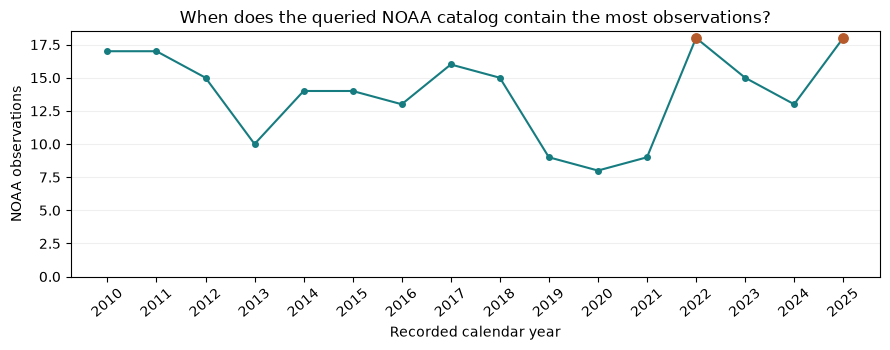
\includegraphics[width=\textwidth]{figures/noaa_tsunami_observations_by_year.png}
\caption[Annual NOAA tsunami observations]{Yearly observation counts in the queried NOAA HazEL subset. The highlighted points mark the years with the most records.}
\label{fig:noaa-annual}
\end{figure}

\subsection{Earthquake Magnitude and Water Height}
The bivariate analysis pairs two measurements from each NOAA record. It selects cause code~1 (earthquake only) and excludes entries marked erroneous or seiche-only. Of 179 selected observations, 172 have both finite measurements. Spearman correlates the paired ranks, with average ranks for ties \cite[PDF p.~20]{edaguide}.

\begin{figure}[htbp]
\centering
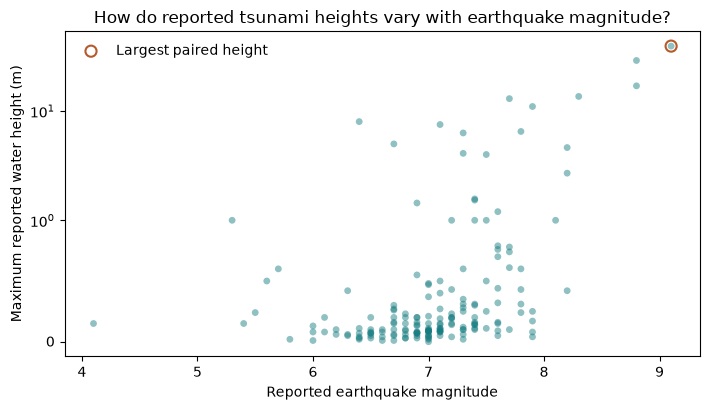
\includegraphics[width=.9\textwidth]{figures/noaa_magnitude_water_height.png}
\caption[Reported earthquake magnitude and maximum water height]{Earthquake magnitude and maximum reported water height in the 172 complete NOAA pairs. The axis is logarithmic above 1~m. The outlined point is the largest paired height (39.26~m).}
\label{fig:noaa-magnitude-height}
\end{figure}

The rank association is positive ($\rho=0.471$), with substantial variation in heights at similar magnitudes (\cref{fig:noaa-magnitude-height}). Omitting the largest paired height in a sensitivity check gives $\rho=0.462$. The full analysis retains that point. The complete pairs represent a subset of the queried catalog, and causal attribution and height prediction require further evidence.

\chapter{PySpark Implementation}
\label{ch:pyspark}
\section{Spark Session and Docker Configuration}
PySpark is the Python interface to Apache Spark. The project uses its DataFrame API to read several Parquet files per topic, select one version of each observation, and group the selected rows into indicators. The Airflow image includes Java~17 and PySpark~3.5.3. \path{src/spark_session.py} creates a local session with configurable defaults of two execution threads, 1~GiB of driver memory and four shuffle partitions. It uses UTC and reads compatible schemas across files. Docker Compose mounts the existing Silver and Gold directories \cite{spark353,pyspark,parquet,compose}.

\section{Gold DAG}
The \path{gold_processing} DAG runs daily at 06:00 UTC with catchup disabled and permits manual runs. Its \path{build_gold} task starts one Spark session, calls \path{src/gold.py}, records the input and output counts and stops the session. The completed pair is published to \path{datalake_gold/} under one UTC stamp. Each Parquet dataset is a directory with its data part and a \path{_SUCCESS} marker. The notebook opens the latest complete pair with the same stamp \cite{airflow}.

\section{Key Transformations}
\label{sec:gold-transforms}
Gold discovers Parquet in the Silver topic directories and in the Workshop~2 flat layout. For legacy files that store timestamps in nanoseconds, it makes temporary microsecond Parquet copies and keeps the original paths for provenance and ordering. The original files remain in Silver. Gold skips empty snapshots and gives wholly untyped rejection identifiers a nullable string type when needed for compatible reads.

For each \path{(source, external_id)} key, Gold ranks earthquake rows by source revision and bulletin rows by Atom update time, using the CAP issue time when Atom time is missing. NOAA and tied revisions use Bronze capture order, with processing time and file information as fallbacks. The path and row values settle remaining ties deterministically. Spark retains the occurrence count and selects one row per key. The flat archives contribute 91 USGS Realtime keys and one PTWC key absent from the topic snapshots. The selected publication consolidates 11,304 USGS Realtime rows into 759 observations. Governance retains the processing totals and quality summaries, and Storytelling aggregates the selected observations.

\chapter{Results}
\label{ch:results}
This chapter combines read-only PostgreSQL results collected at \dbdate, Airflow execution records and local task logs, and the published Gold pair \goldstamp. All timestamps reported as evidence use UTC. The files and queries used to check these results are identified in \cref{app:reproduce}.

\section{Airflow Executions and Incremental Loads}
Airflow recorded 28 successful \path{incremental_ingestion} runs at the metadata check. The project database contained 13 successful incremental source loads, all for USGS Realtime. They read 8,630 observations across their input snapshots and recorded three insertions, four business updates, 8,623 unchanged rows and zero rejections. The counts are processing outcomes across loads. A successful poll can have no manifest, and a committed batch can contain only rows counted as unchanged.

\begin{table}[htbp]
\centering
\small
\begin{tabular}{@{}lrrrrrr@{}}
\toprule
Run ID & \makecell{Finished\\UTC} & Read & New & Updated & Unchanged & Rejected \\
\midrule
18 & 01:11:11 & 664 & 1 & 1 & 662 & 0 \\
19 & 01:21:10 & 664 & 0 & 0 & 664 & 0 \\
28 & 05:21:13 & 663 & 0 & 1 & 662 & 0 \\
\bottomrule
\end{tabular}
\caption[Selected successful USGS Realtime loads]{Selected successful USGS Realtime loads on 20 November 2026, from PostgreSQL \texttt{ingestion\_run}. Times use \texttt{finished\_at}.}
\label{tab:incremental-runs}
\end{table}

\begin{table}[htbp]
\centering
\small
\begin{tabularx}{\textwidth}{@{}L{4.1cm}r r Y@{}}
\toprule
DAG & \makecell{Logical\\time} & \makecell{Finished\\UTC} & Evidence \\
\midrule
\path{incremental_ingestion} & 04:50:00 & 05:00:07 & Success. The publish task reported \emph{nothing new in this run}. \\
\path{incremental_ingestion} & 05:10:00 & 05:20:06 & Success. One candidate from 663 USGS Realtime records. The publish task wrote \path{bronze_manifest_20261120_051000_feeds.json}. \\
\path{silver_processing} & 05:10:00 & 05:21:19 & Success. Loaded that manifest as run~28, reconciled links and cleared the marker. \\
\path{gold_processing} & 04:46:06 & 04:46:54 & Manual run succeeded. \path{build_gold} published the pair \manualgoldstamp. \\
\bottomrule
\end{tabularx}
\caption{Selected Airflow runs on 20 November 2026. The state and times come from Airflow metadata. The artifact and processing descriptions come from task logs. Times are shown to the second.}
\label{tab:airflow-examples}
\end{table}

The \path{load_to_database} log for the 05:10 Silver run records the same counters as run~28 in \cref{tab:incremental-runs}. The \path{publish} log for the 04:50 feed poll provides evidence for the no-change path. Its successful run did not produce a source-load row. The available execution metadata contains no stand-alone FDSN reconciliation run. The FDSN schedule and overlap are verified from code, and the isolated CLI test exercises the watermark-based query.

\section{Canonical Observations and Matching}
\begin{table}[htbp]
\centering
\small
\begin{tabularx}{\textwidth}{@{}lrrY@{}}
\toprule
Source & PostgreSQL & Gold & Committed watermark (UTC) \\
\midrule
NOAA HazEL    & 221   & 221   & No revision watermark \\
USGS FDSN     & 1,929 & 1,929 & 2026-11-19 17:21:44.087 \\
USGS Realtime & 758   & 759   & 2026-11-20 05:12:11.040 \\
NTWC          & 1     & 1     & 2026-11-13 23:30:02 \\
PTWC          & 2     & 2     & 2026-11-18 02:30:47 \\
\midrule
Total         & 2,911 & 2,912 & \\
\bottomrule
\end{tabularx}
\caption[Observation counts and watermarks by source]{Observation counts by source. PostgreSQL counts and watermarks were read at \dbdate. Gold counts come from the publication at \golddate.}
\label{tab:canonical-counts}
\end{table}

PostgreSQL returned zero duplicate \path{(source, external_id)} keys. Its counts matched the earlier Gold pair \manualgoldstamp. The selected Gold pair adds one USGS Realtime observation. A comparison of row values requires a common cutoff.

\begin{table}[htbp]
\centering
\small
\begin{tabular}{@{}lrrrr@{}}
\toprule
Relation type & Accepted & Pending & Rejected & Total \\
\midrule
\path{caused_by} & 163 & 14 & 0 & 177 \\
\path{reports_on} & 0 & 2 & 0 & 2 \\
\path{identity_candidate} & 0 & 0 & 0 & 0 \\
\midrule
Total & 163 & 16 & 0 & 179 \\
\bottomrule
\end{tabular}
\caption{Stored relationships by review status at the read-only PostgreSQL check. All 179 links had rule version~2 in their evidence.}
\label{tab:relations}
\end{table}

Matching produced 177 tsunami-to-earthquake links and two pending bulletin links. Links are counted per pair of observations. The database contained no exact external IDs shared by the two USGS source sets and no identity groups at the check. The grouping behavior is demonstrated with isolated PostGIS fixtures.

\section{Gold Outputs and Notebook}
The published pair \goldstamp{} contains six Governance rows and 96 Storytelling rows. \Cref{tab:gold-quality,tab:story-counts} summarize the two datasets, and \cref{app:samples} gives example rows. The notebook uses Storytelling for the magnitude heatmap and consolidated Silver records for the NOAA figures.

\begin{table}[htbp]
\centering
\small
\begin{tabularx}{\textwidth}{@{}Yrr@{}}
\toprule
Storytelling metric & Parquet rows & Sum of observation counts \\
\midrule
Earthquakes by year & 17 & 2,688 \\
Historical tsunamis by year & 16 & 221 \\
Earthquake magnitude distribution & 37 & 2,688 \\
Maximum tsunami water-height distribution & 24 & 209 \\
Bulletins by center & 2 & 3 \\
\midrule
Total Parquet rows & 96 & \\
\bottomrule
\end{tabularx}
\caption{Storytelling coverage in the selected pair. Each metric has its own denominator and can describe observations also represented in another metric.}
\label{tab:story-counts}
\end{table}

\section{Automated Checks and Command-Line Validation}
The Workshop~3 suite passed 33 local tests with isolated PostgreSQL/PostGIS and eight Airflow and Spark tests in the project image. The checks cover replay, revisions, load rollback, review behavior, marker recovery and reading Gold. The notebook produced identical results from the repository root and \path{notebooks/}. Checks covered incomplete Gold pairs, the Silver fallback and a two-pair sample with a legacy duplicate. Independent NumPy and SciPy calculations verified the statistics and Spearman coefficient.

The current \path{ingest.py} reuses extraction, Silver, PostgreSQL loading and matching. The verified command-line scope is a one-day historical run with local HTTP fixtures against isolated PostGIS, repeated incremental polls, source errors, exit codes and a read-only status request to the project database. Repeating the fixture historical load preserved two observations, and replaying the same incremental response preserved the committed watermarks and observation count. A revised fixture updated the existing observation. The full historical date range was outside the validation scope.

\paragraph{Pending submission evidence.}
Attach Airflow Grid or task-log screenshots for the selected incremental, Silver and Gold executions in \cref{tab:airflow-examples}. Include the two published Parquet samples if the submission requires checked-in Gold artifacts. The tables document the verified execution and dataset results for this draft.

\chapter{Discussion}
The Gold pair captures what was present in the saved Silver files at its publication time. Realtime contributes observations from a rolling feed captured in snapshots, while FDSN and HazEL apply historical and geographic filters. Bulletin counts reflect the few CAP messages captured from the two feeds. Official centers can publish several messages for one episode, and a missed feed window can limit coverage.

Matching depends on the supplied times, locations and magnitudes. Incomplete NOAA records have wider time windows and can require review. A CAP origin time reported inconsistently can prevent a link under the configured time rule, even when a plausible nearby earthquake exists. Earlier profiling documented such a case. Automated acceptance supports triage under the project's rules. Independent review remains necessary for scientific attribution and operational decisions \cite{workshop1,teamassignment}.

The four largest NOAA heights carry the landslide cause code. This pattern suggests an exploratory hypothesis that the upper tail of reported heights differs by documented cause. Assessing it would require comparable measurements and case-level evidence about how the heights were recorded.

Historical and recent comparisons in Workshop~4 should state the observation windows and harmonize thresholds for any rate comparison. The full monitoring interface and tsunami-relevance indicator belong to that stage. The Workshop~3 datasets provide source coverage, quality evidence, and descriptive context for that work \cite{courseproject}.

\chapter{Conclusions and Open Questions}
Workshop~3 connects scheduled source polling to a transactional canonical load and a separate analytical Gold layer. The recorded incremental runs show insertion, revision, and replay outcomes for observations identified by source and external ID. The selected Gold publication counts 2,912 observations across five sources. The PostgreSQL check at an earlier cutoff counts 2,911.

The 32 NOAA records with incomplete clocks support yearly counts and require wider windows for matching. The median and IQR describe the centre of a height distribution with a long upper tail. The positive magnitude--height association describes the complete earthquake-caused pairs, whose heights vary even at similar magnitudes. The dashboard stage still needs to decide how to communicate link confidence and source coverage alongside the historical baseline.

\section{Reflection}
The team separated processing volume from the number of current observations after inspecting repeated Silver snapshots. The flat Workshop~2 archives contained source observations missing from the topic-only scan, and their timestamp representation needed a compatibility read. Including the archives with version selection preserved coverage and the original files. The verification also showed why the time of a poll, the commit time and the Gold publication time belong in separate columns. Each records a different stage of the workflow.

    % -------------------------------------------------------------------
    % References
    % -------------------------------------------------------------------
\begin{thebibliography}{99}
\small
\raggedright
\setlength{\bibsep}{2pt}
\bibitem{hazel} National Geophysical Data Center / World Data Service. \emph{NCEI/WDS Global Historical Tsunami Database}. NOAA National Centers for Environmental Information. doi:10.7289/V5PN93H7. Accessed through the HazEL API, \url{https://www.ngdc.noaa.gov/hazel/view/swagger}, 8 November 2026.
\bibitem{usgsfdsn} U.S.\ Geological Survey. \emph{API Documentation -- Earthquake Catalog}. \url{https://earthquake.usgs.gov/fdsnws/event/1/}. Accessed 8 November 2026.
\bibitem{usgscredit} U.S.\ Geological Survey. \emph{Acknowledging or Crediting USGS}. \url{https://www.usgs.gov/information-policies-and-instructions/acknowledging-or-crediting-usgs}. Accessed 8 November 2026.
\bibitem{usgsfeed} U.S.\ Geological Survey. \emph{Real-time Notifications, Feeds, and Web Services (GeoJSON summary feed)}. \url{https://earthquake.usgs.gov/earthquakes/feed/v1.0/geojson.php}. Accessed 7 and 9 November 2026.
\bibitem{hazelforms} NOAA National Centers for Environmental Information. \emph{HazEL tsunami event search} and \emph{earthquake search} forms. \url{https://www.ngdc.noaa.gov/hazel/view/hazards/tsunami/event-search} and \url{https://www.ngdc.noaa.gov/hazel/view/hazards/earthquake/search}. Accessed 16 November 2026.
\bibitem{tsunamigov} NOAA National Weather Service, Tsunami Warning Centers. \emph{Tsunami event feeds}. \url{https://www.tsunami.gov/}. Accessed 7 and 9 November 2026.
\bibitem{marineregions}
Flanders Marine Institute (2021).
\emph{Global Oceans and Seas, version 1}.
Marine Regions.
\url{https://doi.org/10.14284/542}.
Licensed under CC BY 4.0.
Accessed 16 November 2026.

\bibitem{taupo}
Smithsonian Institution, Global Volcanism Program (2022).
\emph{Report on Taupo (New Zealand),
30 November--6 December 2022}.
\url{https://volcano.si.edu/showreport.cfm?gvpvar=GVP.WVAR20221130-241070}.

\bibitem{tracy}
Shugar, D. H., et al.\ (2026).
\emph{A 481 m-high landslide-tsunami in a
cruise ship--frequented Alaska fjord}.
\textit{Science}. doi:10.1126/science.aec3187.
\url{https://doi.org/10.1126/science.aec3187}.
Accessed 16 November 2026.
\bibitem{workshop1} Team 8. \emph{Tsunami Monitoring System -- Workshop No.~1: Hazard Definition, Source Validation, and Data Contract}. Universidad Distrital Francisco Jos\'e de Caldas, 2026. \url{https://github.com/g8martinezsilva/tsunami-monitoring/tree/workshop-1}.
\bibitem{airflow} The Apache Software Foundation. \emph{Apache Airflow 2.10 documentation}. \url{https://airflow.apache.org/docs/apache-airflow/2.10.4/}. Accessed 17 November 2026.
\bibitem{compose} Docker Inc. \emph{Docker Compose documentation}. \url{https://docs.docker.com/compose/}. Accessed 17 November 2026.
\bibitem{postgis} PostGIS Project Steering Committee. \emph{PostGIS documentation}. \url{https://postgis.net/documentation/}. Accessed 17 November 2026.
\bibitem{pandas} The pandas development team. \emph{pandas documentation}. \url{https://pandas.pydata.org/docs/}. Accessed 17 November 2026.
\bibitem{parquet} The Apache Software Foundation. \emph{Apache Parquet documentation}. \url{https://parquet.apache.org/docs/}. Accessed 17 November 2026.
\bibitem{workshop2} Team 8. \emph{Tsunami Monitoring System -- Workshop No.~2: Technical Architecture, Historical Ingestion and Bronze/Silver Pipeline}. Universidad Distrital Francisco Jos\'e de Caldas, 2026. \url{https://github.com/g8martinezsilva/tsunami-monitoring/tree/workshop-2}.
\bibitem{pyspark} The Apache Software Foundation. \emph{PySpark documentation}. \url{https://spark.apache.org/docs/latest/api/python/}. Accessed 17 November 2026.

\bibitem{courseproject} Sierra, C. A. \emph{Course Project Description: Natural Hazard Monitoring Systems}. Data Analysis Programming, Semester 2026-II. Universidad Distrital Francisco Jos\'e de Caldas. Course handout.
\bibitem{teamassignment} Sierra, C. A. \emph{Team Project Assignment: Natural Hazard Monitoring Systems}. Data Analysis Programming, Semester 2026-II. Universidad Distrital Francisco Jos\'e de Caldas. Course handout.
\bibitem{goldguide} Sierra, C. A. \emph{Workshop No.~3: Silver-to-Gold Pipeline, Governance KPIs, and Storytelling Definition}. Data Analysis Programming, Semester 2026-I. Universidad Distrital Francisco Jos\'e de Caldas. Course handout.
\bibitem{edaguide} Sierra, C. A. \emph{Data Engineering and Visualization: ETLs, EDAs, Data Curation, and Visual Storytelling}. Semester 2026-I. Universidad Distrital Francisco Jos\'e de Caldas. Course slides.
\bibitem{spark353} The Apache Software Foundation. \emph{Apache Spark 3.5.3 Documentation}. \url{https://spark.apache.org/docs/3.5.3/}.
\bibitem{postgresql} The PostgreSQL Global Development Group. \emph{PostgreSQL 16 Documentation: INSERT}. \url{https://www.postgresql.org/docs/16/sql-insert.html}.
\bibitem{postgis-distance} PostGIS Project Steering Committee. \emph{PostGIS Reference: ST\_DWithin}. \url{https://postgis.net/docs/ST_DWithin.html}.
\end{thebibliography}

    % -------------------------------------------------------------------
    % Appendices
    % -------------------------------------------------------------------
    \begin{appendices}

\chapter{Gold Sample Records}
\label{app:samples}
The following rows are selected directly from the two Parquet directories with stamp \goldstamp. Columns are projected to keep the examples readable.

\begin{table}[htbp]
\centering
\small
\begin{tabularx}{\textwidth}{@{}Ylrrrrr@{}}
\toprule
Topic & Source & \makecell{Rows\\processed} & Unique & Repeated & \makecell{Rejections\\processed} & \makecell{Rejections\\distinct} \\
\midrule
\path{tsunami_events} & \path{noaa_hazel} & 459 & 221 & 238 & -- & -- \\
\path{rejected_records} & \path{usgs_fdsn} & -- & -- & -- & 2 & 1 \\
\bottomrule
\end{tabularx}
\caption{Selected Governance fields. Dashes represent nulls in the Parquet output.}
\label{tab:sample-governance}
\end{table}

\begin{table}[htbp]
\centering
\small
\begin{tabularx}{\textwidth}{@{}YlYr@{}}
\toprule
Metric & Source & Dimension values & Count \\
\midrule
Earthquakes by year & \path{usgs_fdsn} & 2011 & 186 \\
Historical tsunamis by year & \path{noaa_hazel} & 2022 & 18 \\
Earthquake magnitude distribution & \path{usgs_realtime} & \texttt{mb}, $[4.5,5.0)$ & 508 \\
Maximum tsunami water-height distribution & \path{noaa_hazel} & $[0,1)$~m & 163 \\
Bulletins by center & \path{ptwc} & \texttt{ptwc} & 2 \\
\bottomrule
\end{tabularx}
\caption{Selected Storytelling rows. The dimension column combines the populated grouping values for each metric.}
\label{tab:sample-story}
\end{table}

\chapter{Reproducing the Workshop 3 Results}
\label{app:reproduce}
\section{Read Published Results}
Run \path{notebooks/03_data_quality.ipynb} with the project kernel from the repository root or \path{notebooks/}. Use the saved Silver inputs and verify Gold stamp \goldstamp. Set \path{SILVER_DIR} and \path{GOLD_DIR} to use archived inputs. With the PostgreSQL settings from the README, inspect the current database state using the status command.

\begin{lstlisting}[language=bash,numbers=none]
python ingest.py --mode status
\end{lstlisting}

Use this read-only SQL in the project database to inspect the load and relationship counts in \cref{ch:results}.

\begin{lstlisting}[language=SQL,numbers=none]
BEGIN ISOLATION LEVEL REPEATABLE READ READ ONLY;
SET LOCAL TIME ZONE 'UTC';
SELECT source, count(*) FROM event GROUP BY source;
SELECT run_id, source_id, status, finished_at, read_count,
       accepted_count, updated_count, unchanged_count,
       rejected_count, input_references
FROM ingestion_run WHERE mode = 'incremental' ORDER BY run_id;
SELECT relation_type, review_status, count(*)
FROM event_relation GROUP BY relation_type, review_status;
ROLLBACK;
\end{lstlisting}

\section{Trace an Execution}
In the Airflow UI, find the runs in \cref{tab:airflow-examples}. Compare the \path{poll_feed}, \path{publish}, \path{find_new_bronze_runs} and \path{load_to_database} logs with \path{ingestion_run.input_references}. Run~28 points to \path{bronze_manifest_20261120_051000_feeds.json}. The manual Gold run \path{manual__2026-11-20T04:46:06.208614+00:00} lists its inputs and outputs in \path{build_gold}.

On an isolated installation, run \path{incremental_ingestion} and \path{silver_processing}, then trigger \path{gold_processing}. See the project READMEs for connection settings and migration.

\paragraph{Automated checks.}
Set \path{TSUNAMI_TEST_DSN} to a disposable PostGIS database. Run from the repository root. Airflow and Spark instructions are in \path{workshop_3/README.md}.

\begin{lstlisting}[language=bash,numbers=none,aboveskip=4pt,belowskip=4pt]
python -B -m unittest discover -s tests -v
\end{lstlisting}

    \end{appendices}

\end{document}
